\phantomsection
\section*{Conceptos básicos}
\addcontentsline{toc}{chapter}{Conceptos básicos}

\phantomsection
\subsection*{Topología}
\addcontentsline{toc}{section}{Topología}

\begin{deff}
    Dado un conjunto $X$, una {\bf topología} $\cT$ sobre $X$ es una colección de subconjuntos de $X$ verificando los siguientes axiomas:

    \begin{enumerate}[leftmargin=15pt,itemsep=0pt, topsep=5pt]
        \item $\emptyset \in \cT$ y $X \in \cT$.
        \item La unión {\it arbitraria} de elementos de la topología da como resultado un elemento de la topología.
        \item La intersección {\it finita} de elementos de la topología da como resultado un elemento de la topología.
    \end{enumerate}
\end{deff}

A los elementos de la topología se les denomina {\it abiertos}, mientras que sus complementarios se denominan \textit{cerrados}. Al par $(X,\cT)$ se le denomina {\it espacio topológico}.

\begin{ejs}
    \item En los números reales $\R$, la colección $\cA = \{(a,b) \mid a,b \in \R \text{ con } a < b\}$ no es una topología sobre $\R$, pues la unión de los intervalos $(0,1)$ y $(2,3)$ no es de nuevo un intervalo.
    \item En los números reales $\R$, la colección $\cT_u$, formada por la unión arbitraria de elementos de $\cA$ junto con el conjunto vacío, sí es una topología, pues se verifica que:
    \begin{enumerate}[itemsep=0pt]
        \item $\emptyset \in \cT_u$, y $\R\in\cT_u$, pues $\R = \bigcup\limits_{n \in \N}(-n,n)$.
        \item La condición de unión arbitraria se ha tomado en la construcción de $\cT_u$.
        \item La intersección finita de intervalos tipo $(a,b)$ resulta en el conjunto vacío o en otro intervalo de la misma forma, por lo que la intersección finita de elementos de $\cT_u$ vuelve a estar en $\cT_u$.
    \end{enumerate}
    A esta topología se le denomina topología usual de $\R$.
    \item En $\topusu$ los conjuntos unipuntuales $\{x\}$ son cerrados, pues sus complementarios, $\R - \{x\}$, son abiertos. De igual manera, los intervalos cerrados $[a,b]$ son cerrados en la topología usual. Por otro lado, los intervalos $[a,b)$ no son abiertos ni cerrados.
\end{ejs}


\phantomsection
\subsection*{Base y subbase de una topología}
\addcontentsline{toc}{section}{Base y subbase de una topología}

\begin{deff}
    Una {\bf base} de una topología $\cT$ es una subcolección $\cB \subset \cT$ tal que todo elemento no vacío de $\cT$ se puede expresar como unión de elementos de $\cB$.
\end{deff}

La noción de base nos permite definir topologías de manera más simple, pues es suficiente con dar los elementos de la base, a los que llamaremos \textit{elementos básicos}. Así, para construir la topología, simplemente hacemos uniones arbitrarias de estos elementos básicos (y añadimos el conjunto vacío si fuera necesario).

\begin{ej}
En la topología discreta en $\R$, la familia de conjuntos unipuntuales $\cB = \{\{x\} \mid x\in \R\}$ es una base de la topología, pues cualquier subconjunto no vacío de $\R$ se puede expresar como unión de conjuntos unipuntuales.
\end{ej}

A veces, probar que una colección de conjuntos es una base puede ser complicado. Para ello se puede usar el siguiente resultado:

\begin{prop}
    {\bf (Caracterización local de base)}
    \item Sea $(X,\cT)$ un espacio topológico y $\cB\subset\cT$. Entonces $\cB$ es una base de $\cT$ si y solo si para cada $x \in X$ y para cada $U \in \cT$ que contiene a $x$, existe un elemento básico $B\in \cB$ tal que $x \in B \subset U$.
\end{prop}

 Esta condición ayuda a reforzar la idea de que los elementos básicos están ``en todos lados'', o que sirven como bloques para construir la topología. Además, si ya se conociera una base $\cA$ de $\cT$, y se tratara de demostrar que otra colección $\cB$ es base, la condición anterior se puede simplificar tomando abiertos de la base $\cA$ en vez de abiertos arbitrarios $U$. En notación lógica se tiene:
    \[(\forall x \in X) (\forall A \in \cA \text{ con } x \in A) (\exists B\in \cB \text{ con } x \in B \subset A)\]
     

\begin{ej}
    En los números reales, la colección $\cA = \{(a,b) \mid a,b \in \R \text{ con } a < b\}$ es una base para la topología usual. Otra base para esta topología es la formada por los intervalos con extremos racionales: $\cB = \{(p,q) \mid p,q \in \Q \text{ con } p < q\}$. Para comprobar que efectivamente es una base, nos valemos del último resultado: para cada $x \in \R$ y $A = (a,b) \in \cA$ con $a < x < b$, como entre dos números reales cualesquiera existen números racionales, se tiene que $ a < p < x < q < b$, con $p,q \in \Q$. Así, existe un elemento $B = (p,q) \in \cB$ con $x \in B \subset A$ y se concluye que $\cB$ también es base.
\end{ej}

Se puede simplificar aún más cómo se presenta una topología mediante el concepto de {\bf subbase}.

\begin{deff}
    Una {\bf subbase} de una topología $\cT$ es una subcolección $\cS\subset\cT$ tal que la colección formada por todas las intersecciones finitas de elementos de $\cS$ es una base de $\cT$.
\end{deff}

Se aprecia que la unión de los elementos de la subbase debe ser el espacio total $X$, pues si no, habría algún elemento $x\in X$ sin que ningún elemento básico de $\cT$ lo contuviera, contra la caracterización dada de elemento básico.

\begin{ejs}
    \item En los números reales, la colección de rayos $\cS = \{(-\infty,b) \mid b \in \R\} \cup \{(a, \infty) \mid a \in \R\}$ es una subbase para la topología usual. Se aprecia que la intersección de dos elementos cualesquiera de $\cS$ es de nuevo o un rayo, o el vacío, o un intervalo $(a,b)$. Así, se puede formar una nueva base de la topología usual tomando estas intersecciones.
    \item En $\R$ se puede generar la topología discreta mediante la subbase $\cS = \{[a,b] \mid a,b \in \R \text{ con } a < b\}$, pues se aprecia que la intersección de dos elementos $[a,b]$ y $[b,c]$ da como resultado $\{b\}$, obteniéndose que los conjuntos unipuntuales son abiertos (elementos de la base generada por $\cS$).
\end{ejs}

\begin{ex}
    En el conjunto \(\R\) de los números reales, definimos \(\cT\) como la topología definida por la subbase \[\cS = \{[a,b] \mid a, b \in \Q, a < b\}.\]
    Encontrar una base de \((\R,\cT)\) y estudiar si \(\cT_u \subset \cT\).
\end{ex}

\phantomsection
\subsection*{Segundo axioma de numerabilidad}
\addcontentsline{toc}{section}{Segundo axioma de numerabilidad}

Que un espacio topológico satisfaga el {\bf segundo axioma de numerabilidad} ({\bf 2AN}) significa que este contiene una base numerable. Ya sabemos cómo comprobar que cierta colección sea base de una topología, así que nos queda estudiar la numerabilidad.

\begin{deff}
    Un conjunto es {\bf numerable} si es finito o es infinito numerable.
\end{deff}

\begin{deff}
    Un conjunto $\cB$ es {\bf infinito numerable} si existe una función biyectiva $f$ de este a los naturales:
    \[f: \cB \longrightarrow \N\]
\end{deff}

Encontrar tal función biyectiva suele ser tedioso, por lo que se suele usar el siguiente resultado:

\begin{prop}
    {\bf (Caracterización de conjunto numerable)}
    \item Sea $\cB$ no vacío. Entonces, que $\cB$ sea numerable es equivalente a cualquiera de las siguientes condiciones:
    \begin{enumerate}[label=\roman*)]
        \item Existe un conjunto numerable $N$ y una función inyectiva $g: \cB \to N$.
        \item Existe un conjunto numerable $N$ y una función sobreyectiva $h: N \to \cB$.
    \end{enumerate}
    La idea es la siguiente: si existe tal función inyectiva $g$ de $\cB$ a $N$, entonces $\cB$ tiene ``como mucho'' tantos elementos como $N$, pues dos elementos diferentes se mapean en elementos diferentes de $N$, y como $N$ es numerable, $\cB$ también deberá serlo. Por otro lado, la existencia de la función sobreyectiva $h$ de $N$ a $\cB$ implica que $N$ tiene ``como mínimo'' tantos elementos como $\cB$, pues todos los elementos de $\cB$ tienen preimagen por $h$, y así, $\cB$ vuelve a tener ``como mucho'' tantos elementos como $N$.
\end{prop}

Ejemplos de conjuntos numerables que serán útiles en la práctica son:
\begin{enumerate}[topsep=5pt,label=--, itemsep=0pt]
    \item Los números enteros $\Z$.
    \item Los números racionales $\Q$.
    \item Subconjuntos de conjuntos numerables.
    \item Uniones numerables de conjuntos numerables.
    \item Productos finitos de conjuntos numerables.
\end{enumerate}

\begin{ej}
    {\bf (Topología usual de $\R$)} 
    \item Los números reales $\R$ con su topología usual es 2AN: la base $\cB = \{(p,q) \subset \R \mid p,q \in \Q \text{ con } p < q\}$ de intervalos racionales es numerable. Para comprobarlo, basta con encontrar una función inyectiva $g$ de $\cB$ a un conjunto numerable. Tomando $p,q \in \Q$ con $p < q$ se tiene:
    \[
    \begin{array}{rcl}
        g \colon & \cB  & \longrightarrow \Q \times \Q \\
                & (p,q) & \longmapsto     (p,q)
    \end{array}
    \]
    De esta manera, $g$ asigna a cada intervalo $(p,q)$ de $\R$ el par formado por $p$ y $q$ de $\Q$. La función está bien definida, pues asigna a cada elemento de $\cB$ uno de $\Q \times \Q$; y es inyectiva, pues intervalos diferentes producen pares diferentes. Además, como $\Q \times \Q$ es producto finito de conjuntos numerables, es numerable, por lo que se concluye que $\R$ es 2AN.
\end{ej}

Por otro lado, para demostrar que un conjunto $\cB$ no es numerable es suficiente con demostrar que no existe dicha función inyectiva $g\colon \cB \to N$, o la correspondiente función sobreyectiva $h\colon N \to \cB$. Esto también suele ser una tarea difícil, por lo que lo más simple suele ser usar la siguiente caracterización:
\begin{prop}
    {\bf (Caracterización de conjunto no numerable)}
    \item Si existe una función inyectiva $f$ de un conjunto no numerable $K$ a nuestro conjunto $\cB$ a estudiar, entonces $\cB$ no es numerable.
    \item La razón es que si $\cB$ fuera numerable, se tendría que $f$ sería una función inyectiva con codominio numerable, por lo que debería ser $K$ numerable, resultando en una contradicción.
\end{prop}

Así pues, algunos conjuntos no numerables que se utilizarán en la práctica son:
\begin{enumerate}[label=--, itemsep=0pt]
    \item Los números reales $\R$.
    \item Cualquier conjunto que contenga a un conjunto no numerable.
    \item Producto de conjuntos no numerables.
    \item Las partes de un conjunto infinito.
    \item Conjuntos no numerables a los que se les ha quitado una cantidad numerable de elementos, por ejemplo, $\Irr = \R - \Q$.
\end{enumerate}

La demostración de que un espacio topológico no es 2AN se puede abordar mediante demostración directa: el objetivo será demostrar que cualquier base de la topología contiene una subcolección no numerable. Para ello, se toma alguna de las caracterizaciones vistas de base de una topología para construir un subconjunto suyo, el cual se probará luego que es no numerable.

% \begin{enumerate}[label=\alph*)]
%     \item Por demostración directa: El objetivo es demostrar que cualquier base de la topología contiene una subcolección no numerable. Para ello, se toma alguna de las caracterizaciones vistas de base de una topología para construir un subconjunto suyo, el cual se probará luego que es no numerable.
%     \item Por reducción al absurdo: Suponer que existe una base numerable y llegar a una contradicción, generalmente, que la base en sí no cumpla las propiedades de ser base, o que la base no sea realmente numerable.
% \end{enumerate} 


\begin{ej}
    {\bf (Topología de Sorgenfrey)} 
    \item El espacio topológico $(\R, \cT)$, con $\cT$ dada a partir de la base $\cA = \{[a,b) \mid a,b \in \R \text{ con } a < b\}$, no es 2AN.\smallskip

    Se demostrará que toda base de $\cT$ no es numerable mediante los siguientes pasos:

    \begin{enumerate}[topsep=0pt,itemsep=0pt]
        \item Construir una colección $\cC$ cuyos elementos están contenidos en cualquier base.
        \item Probar que los elementos de $\cC$ son distintos (no se repiten).
        \item Demostrar que $\cC$ no es numerable.
        \item Concluir que toda base contiene una subcolección no numerable, y es por lo tanto no numerable.
    \end{enumerate}

    \begin{enumerate}[topsep=5pt,itemsep=0pt]
        \item Sea $\cB$ una base cualquiera de $\cT$. Se tiene entonces que para cada $x\in \R$ y para cada elemento básico $A_x \in \cA$ que contiene a $x$, existe un elemento básico $B_x \in \cB$ con $x \in B_x \subset A_x$. El proceso mental para construir $\cC$ es el siguiente:
        \begin{enumerate}[topsep=2pt]
            \item Tomamos una cantidad no numerable de $x$.
            \item Para cada $x$ elegimos un elemento $A_x$ de forma adecuada.
            \item Por ser $\cB$ base, existirá algún elemento $B_x$ con $x \in B_x \subset A_x$.
            \item Elegimos como elemento de $\cC$ el propio $B_x$, y así, $\cC \subset \cB$.
        \end{enumerate}
        Aplicándolo de forma explícita al problema:
        \begin{enumerate}[topsep=2pt]
            \item Tomamos $x\in \R$, que es no numerable.
            \item Para cada $x$ elegimos un elemento de la forma $A_x = [x,x + 1)$.
            \item Por ser $\cB$ base, existirá algún elemento $B_x$ con $x \in B_x \subset [x,x + 1)$.
            \item Elegimos como elemento de $\cC$ el propio $B_x$, y así, $\cC = \{B_x \mid  x\in \R\}$.
        \end{enumerate}

        \item Hemos de probar que si $x \neq y$, entonces $B_x \neq B_y$. Si $x \neq y$, se puede suponer $x < y$, y es $A_x = [x,x + 1)$ y $A_y = [y,y + 1)$, con $x\in B_x \subset A_x$ e $y\in B_y \subset A_y$. Sin embargo, $x$ no puede pertenecer a ningún subconjunto de $A_y$ por ser $x < y$, por lo que $B_y \not\ni x$, y por lo tanto $B_x \neq B_y$. 
        \item Sabemos de antemano que $\cC$ no es numerable, pues la hemos construido mediante una aplicación inyectiva $f\colon \{A_x\}_{x\in \R} \to \cC\colon A_x \mapsto B_x$, y $\{A_x\}_{x\in \R}$ es no numerable pues $f'\colon \R \to \{A_x\}_{x\in \R} \colon x \mapsto [x,x+1)$ es una función inyectiva con dominio no numerable.
        \item Como toda base $\cB$ de $\cT$ contiene una subcolección $\cC$ no numerable, se concluye que toda base es no numerable, y por consiguiente, $(\R, \cT)$ no es 2AN.
    \end{enumerate}

    \underline{Comentarios}: 
    \begin{enumerate}[topsep=5pt,label=--]
        \item La elección de los $A_x$ de la forma $[x,x+1)$ es uno de los pasos clave. Si se hubieran tomado como $A_x$ abiertos de la forma $[x-\varepsilon, x + 1)$, no se podría asegurar que $B_x \neq B_y$, pues tomando $y = x + \delta$, con $0 < \delta < \varepsilon$, %
        %min{\varepsilon,1}, no lo pongo para no complicar, aunque quizás es obvio
        se puede elegir $B = [x, x+1) \in\cB$, el cual satisface $x\in B \subset A_x$ e $y\in B \subset A_y$, y de esta manera, no se puede asegurar que $\cC$ vaya a ser no numerable, pues la función $f$ que asigna cada $A_x$ con un $B_x$ no sería inyectiva, pues un elemento $B\in\cC$ pasaría a ser imagen de distintos $A_x$.
        \begin{center}
            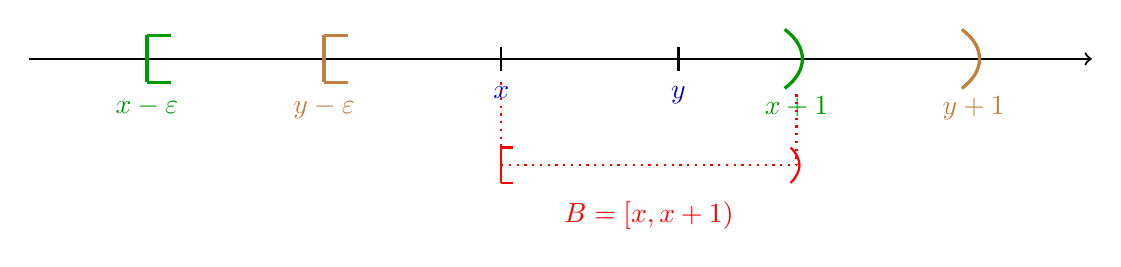
\begin{tikzpicture}[scale=1.5, thick]
                % Recta principal
                \draw[->] (-1, 0) -- (8, 0);

                % Coordenadas de los puntos
                \def\xeps{0}
                \def\yeps{1.5}
                \def\x{3}
                \def\y{4.5}
                \def\xone{5.5}
                \def\yone{7}

                % Puntos en la recta
                \foreach \pos/\label in {\x/x, \y/y} {
                    \draw (\pos, 0.1) -- (\pos, -0.1) node[below=2pt, text=blue!80!black] {$\label$};
                }

                % Intervalo A_x (Verde)
                \draw[green!60!black, very thick] (\xeps, -0.2) -- (\xeps, 0.2);
                \draw[green!60!black, very thick] (\xeps, 0.2) -- (\xeps+0.2, 0.2);
                \draw[green!60!black, very thick] (\xeps, -0.2) -- (\xeps+0.2, -0.2);
                \node[green!60!black, below=10pt] at (\xeps, 0) {$x-\varepsilon$};

                % Paréntesis A_x (Corregido con curva suave)
                \draw[green!60!black, very thick] (\xone-0.1, 0.25) .. controls (\xone+0.1, 0.1) and (\xone+0.1, -0.1) .. (\xone-0.1, -0.25);
                \node[green!60!black, below=10pt] at (\xone, 0) {$x+1$};

                % Intervalo A_y (Marrón)
                \draw[brown, very thick] (\yeps, -0.2) -- (\yeps, 0.2);
                \draw[brown, very thick] (\yeps, 0.2) -- (\yeps+0.2, 0.2);
                \draw[brown, very thick] (\yeps, -0.2) -- (\yeps+0.2, -0.2);
                \node[brown, below=10pt] at (\yeps, 0) {$y-\varepsilon$};

                % Paréntesis A_y (Corregido con curva suave)
                \draw[brown, very thick] (\yone-0.1, 0.25) .. controls (\yone+0.1, 0.1) and (\yone+0.1, -0.1) .. (\yone-0.1, -0.25);
                \node[brown, below=10pt] at (\yone, 0) {$y+1$};

                % Líneas punteadas de conexión para el intervalo B
                \draw[red, thick, dotted] (\x, -0.2) -- (\x, -0.9);
                \draw[red, thick, dotted] (\xone, -0.3) -- (\xone, -0.9);
                \draw[red, thick, dotted] (\x, -0.9) -- (\xone, -0.9);
                
                % Corchete izquierdo del intervalo B
                \draw[red, thick] (\x, -0.75) -- (\x, -1.05);
                \draw[red, thick] (\x, -0.75) -- (\x+0.1, -0.75);
                \draw[red, thick] (\x, -1.05) -- (\x+0.1, -1.05);
                
                % Paréntesis derecho del intervalo B
                \draw[red, thick] (\xone-0.05, -0.75) .. controls (\xone+0.05, -0.85) and (\xone+0.05, -0.95) .. (\xone-0.05, -1.05);

                % Etiqueta
                \node[red, below=3pt] at ({(\x+\xone)/2}, -1.05) {$B = [x, x+1)$};
            \end{tikzpicture}
            \end{center}
        \item La caracterización de base utilizada dice que para cada $x,y$, con $x \neq y$, existen $B_x$ y $B_y$ con $x\in B_x$ e $y\in B_y$, pero no se menciona que dichos elementos básicos deban ser distintos, como se ha visto en el apartado anterior. Es por esto que hay que estudiar la ``no repetición'' de elementos de $\cC$, la cual se consigue mediante una elección adecuada de los abiertos $A_x$.
    \end{enumerate}
\end{ej}

\phantomsection
\addcontentsline{toc}{subsection}{Ejercicios}


\begin{ex}
    En el conjunto \(\mathbb{R}\) de los números reales se considera la topología
    \[
        \cT = \{\emptyset\} \cup \{A \subset \mathbb{R} \mid \mathbb{Q} \subset A\}.
    \]
    Estudiar si \((\mathbb{R}, \cT)\) verifica el segundo axioma de numerabilidad.
    \bigskip

    \textbf{Solución:}
    
    En cualquier ejercicio, lo primero es estudiar cómo se comporta la topología, es decir, qué forma tienen los abiertos o cerrados de esta. Así se podrá intuir hacia dónde van los tiros y proceder adecuadamente. Para ello, consideraremos varios conjuntos, cada vez más complejos, que puedan pertenecer a la topología (ser abiertos).

    Se tiene $\{A \subset \mathbb{R} \mid \mathbb{Q} \subset A\}$, es decir, los abiertos son subconjuntos arbitrarios de $\R$ que contienen a $\Q$. Por ejemplo, aparte del vacío, el siguiente abierto más simple es el propio $\Q$. Podemos continuar infiriendo abiertos: $U = \Q \cup \{\pi\}$, pues $U$ contiene a $\Q$. Así, llegamos a la conclusión de que cualquier abierto no vacío es de la forma $U = \Q \cup K$, donde $K$ es un elemento de partes de $\Irr$, es decir, cualquier subconjunto de $\Irr$. Debido a que la topología involucra a partes de $\Irr$, nos hace pensar que probablemente no tenga una base numerable, por lo que intentaremos demostrarlo:

    \begin{enumerate}[topsep=5pt, itemsep=0pt]
        \item Sea $\cB$ una base cualquiera de $\cT$. Entonces, para cada $x \in \R$ y para cada abierto $U_x \in \cT$ que contiene a $x$, existe un elemento básico $B_x\in\cB$ con $x\in B_x \subset U_x$. Tomemos específicamente los $x$ en $\Irr$ y, como abierto que contiene a $x$, $U_x = \Q \cup \{x\}$. Como $B_x$ es un abierto, será de la forma $B_x = \Q \cup K$, $K\in\cP(\Irr)$, el cual debe contener a $x$ y estar contenido en $\Q \cup \{x\}$, por lo que la única posibilidad es que $B_x = U_x$. Sea por lo tanto $\cC = \{B_x \mid x\in \Irr\} \subset \cB$.
        \item Es trivial que si $x\neq y$ es $B_x \neq B_y$, pues cada uno contiene un irracional que no está contenido en el otro.
        \item De esta forma, $\cC$ es no numerable por existir una función inyectiva $f\colon \Irr\to\cC \colon x \mapsto B_x$.
        \item Como toda base $\cB$ contiene una subcolección no numerable $\cC$, $(\R,\cT)$ no es 2AN.
    \end{enumerate}
\end{ex}

\begin{ex}
    Dado el conjunto \(\mathbb{R}\) de los números reales, se considera la topología 
    \[
        \cT = \{\emptyset\} \cup \{G \subset \mathbb{R} \mid 0 \in G\}.
    \]
    Estudiar si \((\mathbb{R},\cT)\) verifica el segundo axioma de numerabilidad.
    \bigskip

    \textbf{Solución:}

    Los abiertos no vacíos de la topología son conjuntos arbitrarios de $\R$ que contienen al $0$. Por ejemplo, $\{0\}, \{0,5,\pi\}, \Z, \Q$ son abiertos. Vemos de nuevo que esta topología involucra a partes de $\R$, pues todo abierto no vacío se puede expresar de la forma $U = \{0\} \cup K$, con $K \in \cP(\R)$. Por este motivo, se empezará intentando demostrar que no es 2AN:

    \begin{enumerate}[topsep=5pt, itemsep=0pt]
        \item Sea $\cB$ una base cualquiera de $\cT$. Entonces, para cada $x \in \R$ y para cada abierto $U_x \in \cT$ que contiene a $x$, existe un elemento básico $B_x\in\cB$ con $x\in B_x \subset U_x$. Tomemos $x\in \R -\{0\}$ y $U_x = \{0,x\}$ como abierto que contiene a $x$. De esta manera, la única opción posible es que sea $B_x = U_x$, pues debe estar contenido en $U_x$ y contener a su vez a $0$ y $x$. Sea por lo tanto $\cC = \{B_x \mid x\in  \R -\{0\}\} \subset \cB$.
        \item Si $x\neq y$ es evidente que $B_x \neq B_y$.
        \item De esta forma, $\cC$ es no numerable por existir una función inyectiva $f\colon \R -\{0\}\to\cC \colon x \mapsto B_x$ de un conjunto no numerable a $\cC$.
        \item Como toda base $\cB$ contiene una subcolección no numerable $\cC$, $(\R,\cT)$ no es 2AN.
    \end{enumerate}

\end{ex}

\begin{ex}
    \label{Ejercicio:Rcof_irracionales}
    Se considera el espacio topológico \((\mathbb{R}, \cT)\), donde
    \[
        \cT = \{\emptyset\} \cup \{M \subset \mathbb{R} \mid \mathbb{Q} - M \text{ es un conjunto finito}\}.
    \]
    Estudiar si \((\mathbb{R}, \cT)\) verifica el segundo axioma de numerabilidad.

    \bigskip

    \textbf{Solución:}

    Esta vez, los abiertos no vacíos parecen aún más abstractos o difíciles de imaginar. Vayamos entonces identificándolos poco a poco. Los abiertos deben ser subconjuntos $M$ de $\R$ tales que al quitar de $\Q$ los elementos de $M$, el resultado sea un conjunto finito. Veamos:

    \begin{enumerate}[topsep=5pt, itemsep=0pt, label=--]
        \item Si $M$ es finito, será $\Q - M$ infinito, y se deduce que $M$ debe ser infinito.
        \item Sea $M = \Z$. Se vuelve a tener que $\Q - \Z$ es infinito, por lo que $M$ deberá ser ``casi'' $\Q$, para que la diferencia dé como resultado un conjunto finito.
        \item Sea $M = \Q - \{1,2,3\}$. Se obtiene $\Q - M = \{1,2,3\}$ finito, por lo que $\Q - \{1,2,3\}$ es un abierto. De esta manera, se deduce que los conjuntos de la forma $M = \Q - F$ donde $F$ es finito, son abiertos de la topología.
        \item En el apartado anterior, tomando $F = \emptyset$, es $M = \Q - \emptyset = \Q$, y $\Q$ es también abierto ($\Q - M = \emptyset$, que es finito).
        \item ¿Qué sucede si a $\Q$ le quitamos elementos que no están en $\Q$? Por ejemplo, si $M = \Q \cup \{\pi\}$, simplemente será $\Q - M = \emptyset$. De aquí se deduce que añadir elementos irracionales a abiertos no vacíos resulta de nuevo en abiertos. Por ejemplo, $M = (\Q - \{1,2,3, \ldots, 100\}) \cup \{\pi,\pi^2, \pi^3, \ldots\}$ es abierto, pues es $\Q - M = \{1,2,3, \ldots, 100\}$, finito.
        \item Se tiene así que los abiertos no vacíos deben representarse de la forma $U = (\Q - F) \cup K$, con $F \subset \Q$ finito y $K \in \cP(\Irr)$.
    \end{enumerate}

    De nuevo, partes de $\Irr$ está involucrado en la topología, lo que nos hace intuir que no será 2AN:

    \begin{enumerate}[topsep=5pt, itemsep=0pt]
        \item Sea $\cB$ una base cualquiera de $\cT$. Entonces, para cada $x \in \R$ y para cada abierto $U_x \in \cT$ que contiene a $x$, existe un elemento básico $B_x\in\cB$ con $x\in B_x \subset U_x$. Tomemos $x\in \Irr$ y $U_x = \Q \cup \{x\}$ como abierto que contiene a $x$. Un elemento básico $B_x$ que satisfaga $x\in B_x \subset U_x$, se podrá expresar de la forma $B_x = (\Q - F_x) \cup \{x\}$, con $F_x\subset\Q$ finito. Sea entonces $\cC = \{B_x \mid x\in  \Irr\} \subset \cB$.
        \item Si $x\neq y$ es trivial que $B_x \neq B_y$, pues ambos conjuntos contienen un irracional que no pertenece al otro.
        \item De esta forma, $\cC$ es no numerable por existir una función inyectiva $f\colon \Irr\to\cC \colon x \mapsto B_x$ de un conjunto no numerable a $\cC$.
        \item Como toda base $\cB$ contiene una subcolección no numerable $\cC$, $(\R,\cT)$ no es 2AN.
    \end{enumerate}
\end{ex}

\begin{ex}
    \hypertarget{2025 A 2}{}
    En el conjunto \(\mathbb{Z}\) de los números enteros se define la topología \(\cT\) mediante
    \[
        \cT = \{M \subset \mathbb{Z} \mid (0 \notin M) \text{ o } (\mathbb{Z} - M \text{ es finito})\}.
    \]

    Estudiar si \((\mathbb{Z},\cT)\)  verifica el segundo axioma de numerabilidad.
\end{ex}

\begin{ex}
    \hypertarget{2026 A 3}{}
    En el conjunto \(\mathbb{R}\) de los números reales, definimos la topología \(\cT\) mediante \[\cT = \{\emptyset\} \cup \{A \subset \mathbb{R} \mid \mathbb{R} - \mathbb{Q} \subset A\}.\]

    Estudiar si el espacio \((\mathbb{R}, \cT)\) verifica el segundo axioma de numerabilidad.

\end{ex}

\begin{ex}
    \hypertarget{2026 B 3}{}
    Consideremos en el conjunto \(\mathbb{R}\) de los números reales la topología \(\cT\) definida mediante \[\cT = \{A \subset \mathbb{R} \mid 0 \notin A \text{ o } (-1, 1) \subset A\}.\]

    Estudiar si el espacio \((\mathbb{R}, \cT)\) verifica el segundo axioma de numerabilidad.

\end{ex}

\begin{ex}
    \hypertarget{2026 S 3}{}
    En el conjunto \(\R\) de los números reales, definimos \(\cT\) como la topología definida por la subbase \[\cS = \{[a,b] \mid a, b \in \Q, a < b\}.\]

    Estudiar si el espacio \((\mathbb{R}, \cT)\) verifica el segundo axioma de numerabilidad.
\end{ex}


\phantomsection
\subsection*{Entornos en un espacio topológico}
\addcontentsline{toc}{section}{Entornos en un espacio topológico}

\hypertarget{sec:entornos}{}
Dado un espacio topológico $(X,\cT)$, se pueden considerar los elementos de la topología (abiertos $U_x\in\cT$) que contienen a un punto $x\in X$. A su vez, también se pueden considerar los subconjuntos de $X$ que contienen a dichos abiertos $U_x$.

\begin{deff}
    Sea $(X,\cT)$ un espacio topológico.
    \begin{enumerate}[label=--,itemsep=0pt, leftmargin=15pt]
        \item Un {\bf entorno abierto} de $x\in X$ es un elemento de la topología que contiene a $x$.
        \item Un {\bf entorno} de $x\in X$ es un subconjunto de $X$ que contiene a un entorno abierto de $x$.
    \end{enumerate}
\end{deff}

Se deduce que un {\it entorno abierto} de $x$ es a su vez {\it entorno} de $x$, pues se contiene a sí mismo. Generalmente, se hará uso del concepto más general de {\it entorno} a no ser que se quiera especificar que se toma un entorno que es a la vez abierto. Veamos unos ejemplos:

\begin{ejs}
    \item En $(\R,\cT_u)$, el conjunto $U = (-1,1)$ es un entorno de $0$, pues $0\in U$ y $U\in\cT_u$. De esta manera, cualquier subconjunto de $\R$ que contenga a $U$ es también entorno de $0$, por ejemplo, $[-2,\pi)$.
    \item En $(\R,\cT_u)$, el conjunto $\{0\}$ no es un entorno de $0$, pues no puede contener abiertos de $(\R,\cT_u)$ que contengan a $0$, véase, intervalos de la forma $(a,b)$.
    \item En $(\R, \cD)$, los reales con la topología discreta, el conjunto $\{0\}$ {\it sí} es un entorno de $0$, pues el propio $\{0\}$ es un abierto.
\end{ejs}

Podemos considerar la colección $\cE_x$, formada por todos los entornos de un punto $x$. Tal como hemos visto en el ejemplo, esta familia puede ser bastante grande y desordenada, por lo que nos interesa tomar una subcolección $\cA_x \subset \cE_x$ que tenga la propiedad de que, sea cual sea el entorno $E\in \cE_x$ que se tome, existirá un elemento $A\in \cA_x$ contenido en $E$. Formalmente:

\hypertarget{def:base_de_entornos}{}
\begin{deff}
    $\seatop$, $x\in X$ un elemento de $X$, y $\cE_x$ la colección de todos los entornos de $x$. La subcolección $\cA_x \subset \cE_x$ se llama {\bf base de entornos de {\it \textbf{x}}} o {\bf sistema fundamental de entornos de {\it \textbf{x}}} si cualquier entorno $E\in\cE_x$ contiene un elemento $A\in\cA_x$:
    \[\forall E \in \cE_x \ \exists A\in\cA_x \text{ tal que } A \subset E\]
\end{deff}

\begin{ejs}
    \item En $\topusu$, un sistema fundamental de entornos de $0$ es la colección $\cA = \{(-x,x) \mid x \in \R^+\}$. Se aprecia que $\cB = \{[-x,x] \mid x \in \R^+\}$ es también un sistema fundamental de entornos de $0$.
    \item En $(\R, \cD)$, la colección formada por el conjunto $\{0\}$ es un sistema fundamental de entornos de $0$, pues cualquier entorno $E$ de $0$ deberá contener al propio $0$, y es por lo tanto $\{0\}\subset E$.
\end{ejs}

\phantomsection
\subsection*{Primer axioma de numerabilidad}
\addcontentsline{toc}{section}{Primer axioma de numerabilidad}

Que un espacio topológico $(X,\cT)$ satisfaga el {\bf primer axioma de numerabilidad} ({\bf 1AN}) significa que para cada punto $x\in X$ existe un sistema fundamental de entornos numerable. Ya hemos estudiado tanto lo que es un sistema fundamental de entornos en un punto como la numerabilidad, por lo que procedamos a estudiar ejemplos.

\begin{ej}
    {\bf (Topología usual de $\R$)} 
    \item El espacio topológico $\topusu$ es 1AN: la colección $\cA_x = \{(x-q,x+q) \mid q \in \Q^+\}$ es una base de entornos numerable para el punto arbitrario $x\in \R$. Sabemos que es base de entornos de $x$ pues todo entorno $E$ de $x$ debe contener a algún abierto $U_x$ que contenga a $x$, el cual contiene a su vez a un elemento básico $B_x = (x-q,x+q)$, $q \in \Q^+$. Para estudiar la numerabilidad de cada una de estas bases de entornos basta con encontrar una función inyectiva $g_x$ de $\cA_x$ a un conjunto numerable. Sea por lo tanto la función $g_x$ definida como
    \[
    \begin{array}{rcl}
        g_x \colon & \cA_x  & \longrightarrow \Q\\
                & (x-q,x+q) & \longmapsto     q
    \end{array}
    \]
    La función $g_x$ está bien definida, pues asigna a cada elemento $(x-q,x+q)\in\cA_x$ el elemento $q\in\Q$; y es inyectiva, pues si $p = q$, se tiene $(x-p,x+p) = (x-q,x+q)$. Como se ha demostrado que todo punto $x\in\R$ tiene una base de entornos $\cA_x$ numerable, se concluye que $\topusu$ es 1AN.

    \medskip

    \underline{Comentarios}:
    Se puede resolver de igual manera tomando como bases de entornos las colecciones más simples $\cC_x = \{(x-\frac1n,x+\frac1n) \mid n \in \N\}$.
\end{ej}

\bigskip

A diferencia de la demostración de que un espacio topológico no es 2AN mediante demostración directa, la forma más simple de demostrar que un espacio topológico no es 1AN suele ser mediante reducción al absurdo: se busca un elemento $x$ que pueda ser conflictivo y se supone que existe $\cA$, una base de entornos numerable en $x$. Generalmente, la contradicción a buscar será que $\cA$ no sea realmente una base de entornos en $x$, es decir, que exista un entorno $E$ de $x$, de tal manera que no existan elementos $A\in\cA$ contenidos en $E$. Para realizar una demostración por absurdo, lo más conveniente será desarrollar la demostración tanto desde el principio como por el final, e ir hilando y conectando las deducciones que puedan parecer prometedoras. Veámoslo en el siguiente ejemplo.

\begin{ej}
    {\bf (Topología cofinita en $\R$)} 
    \item El espacio topológico $(\R, \cT)$, con $\cT = \{\emptyset\} \cup \{K \subset \R \mid \R - K \text{ es finito}\}$, no es 1AN.\smallskip
    
    El primer paso es estudiar cómo son los abiertos de esta topología, así como sus entornos. Los abiertos no vacíos son de la forma $U = \R - K$, con $K$ finito, pues se necesita que $U$ sea ``casi $\R$'' para que la diferencia sea finita.  Así pues, podemos expresar los abiertos de la forma $U_K = \R - K$ para simplificar. Por otro lado, los entornos serán simplemente subconjuntos de $\R$ que contengan a estos abiertos. Veamos varios ejemplos para hacernos una idea:
    \begin{enumerate}[label=--, topsep=0pt, itemsep=0pt]
        \item $U_{\{1\}}$ es entorno de $0$, pues contiene a todo $\R$ menos al $1$.
        \item $U_{\{1,2,3\}}$ es entorno de $0$, y además es un subconjunto de $U_{\{1\}}$, pues $U_{\{1,2,3\}}$ es todo $\R$ menos dichos $3$ puntos, y $U_{\{1\}}$ es $U_{\{1,2,3\}}$ al que se le ha añadido el $2$ y el $3$.
        \item $U_{\{1,2,3, \pi\}}$ es entorno de $0$, y se tiene la cadena $U_{\{1,2,3,\pi\}} \subset U_{\{1,2,3\}} \subset U_{\{1\}}$. 
        \item $U_{\{2\}}$ es entorno de $0$, sin embargo, se aprecia que no puede ser $U_{\{1\}}\subset U_{\{2\}}$ ni $U_{\{2\}}\subset U_{\{1\}}$, pues ambos contienen un punto que no contiene el otro: $U_{\{1\}}$ contiene el $2$, pero no el $1$, y $U_{\{2\}}$ contiene el $1$ pero no el $2$. Por otro lado, se tiene de nuevo la cadena $U_{\{1,2,3,\pi\}} \subset U_{\{1,2,3\}} \subset U_{\{2\}}$.
        \item Se da así uno cuenta de que $U_B \subset U_C$ si y solo si $C\subset B$.
        \item Además, si $E$ es un entorno de $x$, contendrá a un abierto de la forma $U_K$, con $x\not\in K$, de manera que es $x\in U_K \subset E$. Así, $E$ es un subconjunto de $\R$ que contiene a $U_K$, por lo que deberá ser también de la forma $E = \R - L$, con $L$ un subconjunto de $K$, y se obtiene que $E$ es un abierto. Se concluye por lo tanto que todo entorno de un punto en esta topología es un entorno abierto.
        \item $U_\N$ no es un entorno de $0$, pues $\R - U_\N = \N$, que no es finito, por lo que no es un abierto.
        \item La unión e intersección de abiertos funcionan de manera sencilla: $U_{\{1,2,3\}} \cup U_{\{2,3,4\}} = U_{\{2,3\}}$ y $U_{\{1,2,3\}} \cap U_{\{2,3,4\}} = U_{\{1,2,3,4\}}$. Se tiene simplemente que 
        \[
            \bigcup U_{K_i} = \R - \bigcap K_i
        \]
        \[
            \bigcap U_{K_i} = \R - \bigcup K_i
        \]
        Por ejemplo, 
        \[
            \bigcap\limits_{n\in\N} U_{\{n\}} = \R - \bigcup\limits_{n\in\N} \{n\} = \R - \N = U_\N.
        \]

    \end{enumerate}

    \smallskip

    Habiendo estudiado cómo es la topología y sus operaciones básicas, veamos cómo demostrar que no es 1AN.

    \begin{enumerate}[itemsep=0pt, topsep=0pt, label=--]
        \item Como no parece que haya puntos destacados, tomemos arbitrariamente $0\in\R$ y supongamos que existe una base de entornos numerable en $0$, que llamaremos $\cA$.
        \item Nuestro objetivo es demostrar que $\cA$ no es base de entornos de $0$, es decir, que existe un entorno $E$ de $0$, verificándose $A\not\subset E$, para todo $A\in\cA$. Para ello es suficiente con que exista algún elemento $y\in\R$ tal que $y\in A$ para cada $A\in\cA$ y que $y\notin E$. Debemos por lo tanto escoger un entorno $E$ de manera que no contenga a dicho elemento. ¿Cómo podemos hacer esto, si $\cA$ es arbitraria? ¿Si no se sabe qué elementos tiene? Pues haciendo uso de que es numerable.
        \item Para ello, construyamos $\cA$. Por ser numerable, los elementos de $\cA$ se pueden ordenar de la forma
        \vspace{-1em}
        \begin{align*}
            A_{K_1} = & \ \R - K_1\\
            A_{K_2} = & \ \R - K_2\\
            \vdots&\\
            A_{K_n} = & \ \R - K_n\\
            \vdots&
        \end{align*}
        donde $n\in\N$, y cada $K_n$ es finito y no contiene al $0$ (si $\cA$ fuera finita, simplemente se repite su último elemento indefinidamente para que la expresión tenga sentido).
        \item Queremos encontrar un elemento $y$ que esté en cada $A_{K_n}$. Para ello, tomamos la intersección $A = \bigcap\limits_{n\in\N} A_{K_n} = \R - \bigcup\limits_{n\in\N}K_n$, obteniendo la resta entre un conjunto no numerable y una unión numerable de conjuntos numerables, y es por lo tanto $A$ no numerable. Sea $y\in A - \{0\}$, que existe por ser no numerable, y sea $E = \R - \{y\}$. Se tiene que $E$ es entorno de $0$, sin embargo, ningún elemento $A_{K_n}\in\cA$ está contenido en $E$ pues $y$ pertenece a cada $A_{K_n}$ de $\cA$, pero $y$ no está en $E$.
        \item De esta forma, hemos llegado a la contradicción de que $\cA$ no es una base de entornos de $0$ tras suponer que $\cA$ es numerable, por lo que ha de ser no numerable, y se concluye que $(\R, \cT)$ no es 1AN.
    \end{enumerate}
\end{ej}

Se puede apreciar que en la demostración por absurdo hemos ido desarrollando desde ambos cabos:
\begin{enumerate}
    \item Estudiar la topología y los entornos de puntos.
    \item Suponer la existencia de una base de entornos numerable en un punto.
    \item Deducir cómo se ha de llegar a la contradicción y construir ``hacia atrás'', según cómo se comportan los entornos de la topología (haciendo uso de la definición de base de entornos en un punto).
    \item Construir la base de entornos arbitraria e intentar hilarlo con la contradicción (haciendo uso de la numerabilidad).
\end{enumerate}

Por último, queda resaltar la relación que existe en un espacio topológico entre ser 1AN y 2AN:
\begin{prop}
    Si un espacio topológico es 2AN entonces es 1AN.

    La razón es que simplemente se toman los elementos básicos que sean entornos de un punto, y como es 2AN, la cantidad de los entornos básicos de dicho punto será numerable.
\end{prop}

Podemos deducir por lo tanto que la topología cofinita en $\R$ no es 2AN. 

\phantomsection
\addcontentsline{toc}{subsection}{Ejercicios}

\begin{ex}
    Dado el conjunto \(\mathbb{R}\) de los números reales, se considera la topología 
    \[
        \cT = \{\emptyset\} \cup \{G \subset \mathbb{R} \mid 0 \in G\}.
    \]
    Estudiar si \((\mathbb{R},\cT)\) verifica el primer axioma de numerabilidad.
\end{ex}

\begin{ex}
    Se considera el espacio topológico \((\mathbb{R}, \cT)\), donde
    \[
        \cT = \{\emptyset\} \cup \{M \subset \mathbb{R} \text{ tal que } \mathbb{Q} - M \text{ es un conjunto finito}\}.
    \]
    Estudiar si \((\mathbb{R}, \cT)\) verifica el primer axioma de numerabilidad.
\end{ex}

\begin{ex}
    En el conjunto \(\mathbb{R}\) de los números reales, definimos la topología
    \[
        \cT = \{\mathbb{R}\} \cup \cP(\mathbb{R} - M), \text{ partes de } \mathbb{R} - M, \text{ siendo } M = (1,3).
    \]
    Estudiar si \((\mathbb{R},\cT)\) verifica el primer axioma de numerabilidad.
\end{ex}



\phantomsection
\subsection*{Subconjuntos en un espacio topológico}
\addcontentsline{toc}{section}{Subconjuntos en un espacio topológico}

$\seatop$ y $M\subset X$. Los puntos $x\in X$ se pueden caracterizar mediante abiertos según su relación con $M$. De esta manera, los puntos $x$ se pueden clasificar de manera excluyente y exhaustiva como interiores, exteriores y frontera.

\begin{deff}
    $x$ es un punto \textbf{interior} de $M$ si existe un entorno de $x$ contenido en $M$.
\end{deff}
Al conjunto de todos los puntos interiores de $M$ se le llama \textit{interior} de $M$ y se denotará por \underline{$\interior{M}$}.

\begin{deff}
    $x$ es un punto \textbf{exterior} de $M$ si existe un entorno de $x$ contenido en el complementario de $M$: $X - M$.
\end{deff}
Al conjunto de todos los puntos exteriores de $M$ se le llama \textit{exterior} de $M$ y se denotará por \underline{$\exterior{M}$}.

\begin{deff}
    $x$ es un punto \textbf{frontera} de $M$ si todo entorno de $x$ interseca tanto a $M$ como a $X - M$.
\end{deff}
Al conjunto de todos los puntos frontera de $M$ se le llama \textit{frontera} de $M$ y se denotará por \underline{$\frontera{M}$}.

\begin{ejs}\label{ej:11}
    \item Sea $(\R, \cT)$ con $\cT$ la topología trivial y el conjunto $M = [0,1)\cup \{2\}\subset \R$. Se tiene que 
    \begin{center}
        $\interior{M} = \emptyset;\quad \frontera{M} = \R;\quad \exterior{M} = \emptyset$.
    \end{center}
    \item Sea $\topusu$ y el conjunto $M = [0,1)\cup \{2\}\subset \R$. Se tiene que 
    \begin{center}
        $\interior{M} = (0,1);\quad \frontera{M} = \{0,1,2\};\quad \exterior{M} = \R - ((0,1)\cup \{0,1,2\}).$
    \end{center}
    \item Sea $(\R,\cT)$ con $\cT$ la topología de Sorgenfrey y el conjunto $M = [0,1)\cup \{2\}\subset \R$. Se tiene que 
    \begin{center}
        $\interior{M} = [0,1);\quad \frontera{M} = \{2\};\quad \exterior{M} = \R - ([0,1)\cup \{2\}).$
    \end{center}
    \item Sea $(\R,\cT)$ con $\cT$ la topología discreta y el conjunto $M = [0,1)\cup \{2\}\subset \R$. Se tiene que 
    \begin{center}
        $\interior{M} = [0,1)\cup \{2\};\quad \frontera{M} = \emptyset;\quad \exterior{M} = \R - ([0,1)\cup \{2\})$.
    \end{center}    
\end{ejs}

En los ejemplos anteriores se aprecia que tanto el interior como el exterior de $M$ son conjuntos abiertos, mientras que la frontera es un conjunto cerrado. Además, el exterior no es más que el complementario de unir el interior y la frontera: $\exterior{M} = X - (\interior{M} \cup \frontera{M})$. Por otro lado, se aprecia que los puntos interiores a $M$ pertenecen a $M$, mientras que los puntos frontera pueden o no pertenecer a $M$. \bigskip

Aplicando las definiciones se pueden deducir las siguientes caracterizaciones:
\begin{prop}
    $\seatop$ y $M\subset X$. Entonces se tiene:
    \item -- $M$ es abierto si y solo si no contiene a ninguno de sus puntos frontera.
    \item -- $M$ es cerrado si y solo si contiene a todos sus puntos frontera.
    \item -- $M$ no es ni abierto ni cerrado si y solo si contiene a alguno, pero no todos sus puntos frontera.
\end{prop}
De aquí se obtiene que $M$ es abierto si y solo si $M = \interior{M}$ y que $M$ es cerrado si y solo si $M = \interior{M} \cup \frontera{M}$. A esta última unión se le llama adherencia de $M$.

\hypertarget{def:punto_adherencia}{}
\begin{deff}
    $x$ es un punto \textbf{adherente} a $M$ si todo entorno de $x$ interseca a $M$.
\end{deff}
Al conjunto de todos los puntos adherentes a $M$ se le llama \textit{adherencia} de $M$ y se denota por $\overline{M}$ o por $\operatorname{adh}(M)$. Tal como hemos comentado, se tiene que $\overline{M} = \interior{M} \cup \frontera{M}$, y es por lo tanto $M$ cerrado si y solo si $M = \overline{M}$.

\begin{ex}
    Se considera el espacio topológico \((\mathbb{R}, \cT)\), donde
    \[
        \cT = \{\emptyset\} \cup \{M \subset \mathbb{R} \text{ tal que } \mathbb{Q} - M \text{ es un conjunto finito}\}.
    \]
    Hallar el interior, la adherencia y la frontera del conjunto \(\mathbb{R} - \mathbb{Q}\).

    \bigskip

    {\bf Solución:}

    Tras realizar el análisis del Ejercicio \ref{Ejercicio:Rcof_irracionales}, llegamos a la conclusión de que los abiertos no vacíos de esta topología se pueden representar de la forma $U = (\Q - F) \cup K$, con $F \subset \Q$ finito y $K \in \cP(\Irr)$. Veamos entonces qué puntos son interiores y frontera de $\Irr$, pues la adherencia será su unión.

    Empecemos tomando un punto $x\in\Irr$. Queremos estudiar los entornos de $x$, los cuales contendrán abiertos de la forma $U_x = (\Q - F) \cup \{x\}$. De aquí deducimos que cualquier entorno de $x$ contendrá elementos de $\Q$ y de $\Irr$, por lo que concluimos que $\Irr \subset \frontera{\Irr}$, y su interior será vacío. Nos queda estudiar los puntos $x\in\Q$. Para estos puntos, se pueden tomar entornos de la forma $U_x = \Q$, los cuales están contenidos en el complementario de $\Irr$, y por lo tanto, se concluye que el exterior de $\Irr$ es $\Q$, su interior es vacío, su frontera es el propio $\Irr$, y la adherencia es $\emptyset \cup \Irr = \Irr$.
\end{ex}

\bigskip

En un espacio topológico $(X,\cT)$, los puntos de adherencia de un conjunto $M$ se pueden clasificar según sean puntos de acumulación o puntos aislados.

\begin{deff}
    $x\in X$ es un {\bf punto de acumulación} de $M$ si todo entorno de $x$ interseca a $M$ en un punto distinto a $x$:
    \[\text{Para cada entorno de } x, \ U_x, \text{ se tiene } (U_x -\{x\}) \cap M \neq \emptyset \]
\end{deff}

\begin{deff}
    $x\in M$ es un {\bf punto aislado} de $M$ si existe un entorno de $x$ que no interseca a $M$ en un punto distinto a $x$:
    \[\text{Existe un entorno de } x, \ U_x, \text{ tal que } (U_x -\{x\}) \cap M = \emptyset \]
\end{deff}

\begin{ex}
    Estudiar los puntos de acumulación y los puntos aislados para cada topología del Ejemplo \ref{ej:11}.
\end{ex}


Una propiedad que pueden satisfacer ciertos conjuntos de un espacio topológico es la densidad.

\begin{deff}
    $\seatop$ y $M\subset X$. Se dice que $M$ es {\bf denso} en $X$ si satisface que $\overline{M} = X$.
\end{deff}

La idea es que cualquier abierto no vacío en $X$ contendrá elementos del conjunto denso, tal y como sucede con la topología usual $\topusu$ y el subconjunto $\Q$. Así, una caracterización útil es la siguiente:

\begin{prop}
    $\seatop$ y $M\subset X$. Se tiene entonces que $M$ es denso en $X$ si y solo si para todo abierto no vacío $U\in\cT$ se cumple que \(U \cap M \neq \emptyset\).
\end{prop}

\begin{ex}
    Demostrar la caracterización anterior.
\end{ex}

Los subconjuntos densos en un espacio topológico pueden resultar útiles para estudiar el espacio topológico en sí. Esto se acentúa cuando dicho subconjunto denso es numerable. Los espacios topológicos donde se pueda encontrar dicho conjunto se denominarán separables.

\begin{deff}
    Un espacio topológico es {\bf separable} si contiene un subconjunto numerable y denso.
\end{deff}

Una forma de estudiar si un espacio es separable es estudiando si es segundo numerable:

\begin{prop}
    Si un espacio topológico es 2AN, entonces es separable.
\end{prop}

Veamos varios ejemplos para profundizar los conceptos:

\begin{ejs}
    \item {\bf  $(\R, \cT)$ es separable con la topología de Sorgenfrey}\\
    En $\R$, el prototipo de subconjunto numerable es $\Q$, por lo que veamos si este es denso con esta topología. La forma más simple de demostrar que es separable suele ser usar la caracterización de conjunto denso. Veamos cómo:
    
    Sea $U$ un abierto no vacío. Por ser abierto, existe un elemento básico $B\in\cB$ de la forma $B = [a,b)$, contenido en $U$. Pero entre dos elementos $a,b\in\R$ existe un $q\in\Q$ con $a<q<b$, y por lo tanto $q \in B \subset U$. De esta manera, se ha probado que todo abierto no vacío $U$ contiene elementos de $\Q$ (su intersección no es vacía), y se concluye que $\Q$ es denso en $\R$ con la topología de Sorgenfrey.

    \item {\bf  $(\R, \cT)$ no es separable con la topología discreta}\\
    Al igual que para demostrar que un espacio topológico no es 2AN probando que cualquier base del espacio no es numerable, la no separabilidad se demuestra probando que cualquier conjunto que sea denso no es numerable.

    Empecemos construyendo un subconjunto que sea denso. Sea $M = \{x\}$, con $x\in\R$. Se tiene que $M$ es cerrado, por lo que $\overline{M} = M$. Si en vez de tomar $M = \{x\}$ tomamos $M$ como cualquier subconjunto de $\R$, se tendrá que sigue siendo cerrado por ser su complementario abierto, y es $\overline{M} = M$. De esta forma llegamos a la conclusión de que el único subconjunto denso es el propio $\R$, pues es el único que verificará $\overline{\R} = \R$, y como $\R$ no es numerable, $(\R, \cT)$ no es separable.
\end{ejs}


\phantomsection
\addcontentsline{toc}{subsection}{Ejercicios}

\begin{ex}
    Estudiar si la topología cofinita en $\R$, dada por
    \[
        \cT = \{\emptyset\} \cup \{M\subset\R\mid \R- M \text{ es finito}\},
    \]
    es separable.

    \bigskip

    {\bf Solución:}

    De nuevo, si no supiéramos cómo abordar la demostración, si tirar hacia demostrar que es separable o si tirar hacia que no es separable, primero estudiemos cómo son los abiertos, luego tomemos algún conjunto numerable y estudiemos los entornos de sus puntos y así vamos entendiendo hacia dónde pueden ir los tiros.

    En este caso, se tiene que los abiertos son $\R$ menos un conjunto finito, por lo que tomando un conjunto infinito numerable $M$, cualquier abierto que se tome deberá contener puntos de $M$. Expresándolo de manera formal:

    Sea $U = \R - K$, con $K$ finito, un abierto no vacío y sea $\Z\subset\R$. Se tiene entonces que $U\cap\Z = \Z - K \neq \emptyset$. Al ser $\Z$ numerable y denso, se concluye que $(\R, \cT)$ es separable.
\end{ex}

\begin{ex}
    Estudiar si la topología conumerable en $\R$, dada por
    \[
        \cT = \{\emptyset\} \cup \{M\subset\R\mid \R- M \text{ es numerable}\},
    \]
    es separable.
    
    \bigskip

    {\bf Solución:}

    Si lo intentáramos resolver de la misma manera que el ejercicio anterior, tomando $U = \R - K$, con $K$ un conjunto numerable arbitrario, podría no obtenerse $U\cap\Z = \Z - K \neq \emptyset$, pues tomando $K = \Z$ es $\Z - K = \emptyset$. Estudiemos entonces cómo son los conjuntos numerables respecto a la topología. Si tomamos $M$ numerable, se tiene que $U = \R - M$ es abierto, obteniendo que $M$ es cerrado, por lo que ha de ser $\overline{M} = M$. De esta forma podemos concluir que para todo subconjunto numerable de $\R$, su adherencia es él mismo, distinto de $\R$, y así no existen subconjuntos numerables y densos, por lo que $(\R, \cT)$ no es separable.
\end{ex}

\begin{ex}
    En el conjunto \(\mathbb{R}\) de los números reales se considera la topología
    \[
        \cT = \{\mathbb{R}\} \cup \{G \subset \mathbb{R} \mid 0 \notin G\}.
    \]
    Estudiar si \((\mathbb{R}, \cT)\) es separable.
\end{ex}

\begin{ex}
    En el conjunto \(\R\) de los números reales, definimos \(\cT\) como la topología definida por la subbase 
    \[
        \cS = \{[a,b] \mid a, b \in \Q, a < b\}.
    \]
    Estudiar si \((\R,\cT)\) es separable.
\end{ex}

\phantomsection
\addcontentsline{toc}{section}{Ampliación}

\begin{amp}
    Veamos varios conceptos relacionados con lo estudiado hasta ahora para profundizar en su entendimiento. Empecemos con la relación existente entre las distintas topologías que existen en un conjunto.
    \begin{deff}
        Sean $\cT_1$ y $\cT_2$ dos topologías definidas en $X$. Se dice que $\cT_2$ es {\bf más fina} que $\cT_1$ si $\cT_1\subset\cT_2$.
    \end{deff}
    \begin{ej}
        Se definen en $\R$ las topologías: discreta, $\cD$; Sorgenfrey, $\cS$; usual, $\cT_u$; y trivial $\cT$. Se tiene entonces que $\cT \subset\cT_u \subset\cS \subset\cD$. Esto se puede comprobar 
        mediante la caracterización local de base, donde se toma como abierto arbitrario un elemento de la base más gruesa, es decir, $\cT_2$ es más fina que $\cT_1$ si y solo si
        \[
            (\forall x \in X) (\forall B_1 \in \cB_1 \text{ con } x\in B_1) (\exists B_2 \in\cB_2 \text{ con } x\in B_2 \subset B_1),
        \]
        donde $\cB_1\subset\cT_1$ y $\cB_2\subset\cT_2$ son bases. Por ejemplo, podemos así ver que la topología de Sorgenfrey es más fina que la topología usual de $\R$, pues es trivial encontrar un elemento básico $[c,d)$ en uno $(a,b)$ que contengan a un punto $x$. Por otro lado, se comprueba que la topología usual \textit{no} es más fina que la de Sorgenfrey, pues dado un elemento básico $[a,b)$ que contiene a $x = a$, no existe ningún elemento básico de la usual que contenga a $x$ y que esté contenido en $[a,b)$.
    \end{ej}
    Aunque pueda parecer extraño estudiar de nuevo si una topología $\cT_1$ es más fina que otra, $\cT_2$, habiendo estudiado ya que $\cT_1 \subset \cT_2$, puede darse el caso de que se cumpla que $\cT_1 \subset \cT_2$ y $\cT_2 \subset \cT_1$ cuando ambas topologías sean, de hecho, la misma. Al definir usualmente las topologías mediante bases, puede darse el caso de que bases que parezcan que generan distintas topologías generen de hecho la misma. Es el caso de definir la topología usual mediante abiertos racionales o abiertos reales.

    \bigskip

    Estudiemos ahora las propiedades que cumplen los entornos en un punto, introducidos \hyperlink{sec:entornos}{aquí}. Dado un punto $x\in X$, la colección $\cE_x$ de todos los entornos de $x$ la llamaremos {\bf sistema de entornos de \textit{x}}. Es evidente que al ser $x\in E$ para todo $E\in\cE_x$, \textit{cada elemento de la colección no es vacío}. Por otro lado, la intersección de dos entornos cualesquiera es de nuevo un entorno, pues ambos contendrán abiertos que contengan a $x$, cuya intersección será de nuevo un abierto que contenga a $x$, y es por lo tanto la intersección de entornos un subconjunto que contiene un abierto que contiene a $x$. Con este razonamiento, llegamos a la conclusión de que \textit{la intersección finita de entornos es de nuevo un entorno}. Por último, aunque sea trivial por definición, otra propiedad de los entornos es que \textit{todo subconjunto de $X$ que contenga a un entorno $E$ de $x$ es a su vez un entorno de $x$}. A esta última propiedad se le suele denominar ser cerrado bajo superconjuntos.

    Estas propiedades se pueden generalizar para conjuntos arbitrarios, resultando en una estructura llamada \textit{filtro}, la cual generaliza nociones como los entornos o las sucesiones (que veremos más adelante). En el caso anterior se obtuvo el filtro de entornos en un punto. Así, se puede expresar la definición de filtro como:

    \begin{deff}
        Dado un conjunto $X$, un {\bf filtro} $\cF$ sobre $X$ es una colección no vacía de subconjuntos de $X$ verificando los siguientes axiomas:
        \begin{enumerate}[leftmargin=15pt,itemsep=0pt, topsep=5pt]
            \item $\emptyset \notin \cF$.
            \item La intersección {\it finita} de elementos del filtro es un elemento del filtro.
            \item Es cerrado bajo superconjuntos.
    \end{enumerate}
    \end{deff}

    \begin{ej}
        Tomando como espacio $X = \{1,2,3\}$, la colección $\cF_1 = \{\{1\}, \{1,2\}\}$ no es un filtro pues existen subconjuntos de $X$, véase $\{1,3\}$ y $\{1,2,3\}$, que contienen a elementos de $\cF_1$ y que no pertenecen al filtro. Añadiendo estos conjuntos, se obtiene el filtro $\cF_1 = \{\{1\}, \{1,2\},\{1,3\},\{1,2,3\}\}$.
    \end{ej}

    De igual forma que al definir una topología, un filtro suele ser una familia \textit{muy grande} y desordenada. La forma más conveniente de definirlos es mediante {\it bases de filtro}. 

    \begin{deff}
        Una {\bf base de filtro} de un filtro $\cF$ es una subcolección $\cB\subset \cF$ tal que el filtro $\cF$ se puede obtener tomando superconjuntos de los elementos de la base $\cB$.
    \end{deff}

    De esta manera, una base de filtro $\cB$ no necesita cumplir todas las propiedades de un filtro, sino que se pueden relajar las condiciones a una colección de conjuntos no vacía satisfaciendo:
    \begin{enumerate}[label=--]
        \item $\emptyset \notin \cB$.
        \item La intersección finita de elementos de $\cB$ {\it contiene} a algún elemento de $\cB$.
    \end{enumerate}

    \medskip

    Otra caracterización equivalente de base de filtro es la siguiente:
    \begin{prop}
        $\cB\subset\cF$ es una base de filtro de $\cF$ si y solo si para cada $F\in \cF$ existe un elemento de la base $B\in\cB$ tal que $B\subset F$.
    \end{prop}    
    Ahora podemos ver claramente que la definición de base de entornos en un punto no es más que la base de filtro de entornos en dicho punto (\hyperlink{def:base_de_entornos}{ver la definición de base de entornos en un punto}).

    \begin{ej}
        En los números enteros positivos, $\N$, se puede considerar la colección $\cB$ formada por los conjuntos de la forma $B_n = \{i \mid i \geq n\}$, con $n\geq 1$. Por ejemplo, $B_1 = \{1,2,3,\ldots\}$, $B_2 = \{2,3,4,\ldots\}$, $B_{10} = \{10,11,12,\ldots\}$. Se tiene que $\cB$ es una base de filtro, pues cualquier $B_n$ no es vacío, y la intersección finita de elementos de $\cB$ contiene a un elemento de $\cB$ (por otro lado, se aprecia que la intersección (infinita) de todos los elementos de $\cB$ es el conjunto vacío, que no pertenece a la base). El filtro $\cF$ que genera esta base se forma simplemente añadiendo todos los superconjuntos posibles a los elementos de la base. Por ejemplo, $F = \{2,5,6,7,8,\ldots\}$ es un elemento de $\cF$, pero $F = \{1,3,5,7,\ldots\}$, formado por los impares, no lo es. Se aprecia, al igual que con una topología, que un filtro puede llegar a ser un conjunto extremadamente grande y complejo, de ahí la necesidad de operar usualmente con su base, al igual que sucede con las topologías.
    \end{ej}

    Al igual que se ha hecho con las topologías definidas en un conjunto, se puede estudiar cuándo un filtro es más o menos {\it fino} que otro filtro mediante el uso de sus respectivas bases de filtro. Por ejemplo, en $\R$ con la topología usual y con la topología discreta, se definen sus sistemas de entornos en un punto $x$ (filtros de entornos en $x$), que llamaremos $\cF_{x,U}$ y $\cF_{x,D}$, respectivamente. Una base de entornos en $x$ (base de filtro en $x$) para cada topología es $\cA_x = \{(a,b)\mid a<x<b\}$, para la usual, y $\cB_x = \{\{x\}\}$, para la discreta. Es evidente que para cada $A\in\cA_x$ es $B=\{x\}\subset A$, y así se obtiene que $\cF_{x,U} \subset \cF_{x,D}$. Como cabía esperar, al ser la topología discreta más fina que la usual, su filtro de entornos en un punto es más fino que el de la topología usual. Este resultado se puede generalizar, obteniendo:
    \begin{prop}
        Sean $\cT_1$ y $\cT_2$ dos topologías definidas en $X$. Se tiene entonces que $\cT_2$ es más fina que $\cT_1$ si y solo si, para cada $x\in X$, el filtro de entornos de $x$, $\cF_{x,\cT_2}$, asociado a $\cT_2$, es más fino que el filtro de entornos de $x$, $\cF_{x,\cT_1}$, asociado a $\cT_1$. Expresado de forma compacta:
        \[
            \cT_1\subset\cT_2  \iff \forall x\in X,\ \cF_{x,\cT_1}\subset \cF_{x,\cT_2}.
        \]
    \end{prop}

    \bigskip

    Por último, profundicemos en el concepto de punto de adherencia, introducido \hyperlink{def:punto_adherencia}{aquí}. La adherencia generaliza el concepto de distancia. En un espacio métrico, una función distancia es una forma de medir cuán cerca o cuán lejos están los puntos del conjunto. En un espacio topológico, la forma de ``medir distancias'' es mediante abiertos, concretamente, se usarán entornos en un punto. Así, si para dos puntos $x,y\in X$, todo entorno de $y$ contiene a $x$, $y$ es un punto de adherencia del conjunto unipuntual $\{x\}$, por lo cual $y$ está ``cerca'' de $x$. Podemos entonces considerar el caso de la topología trivial: al solo existir un abierto que contiene a todos los puntos, todos están cerca entre sí; o el de la topología discreta: todos los puntos están ``lejos'', pues cada punto sólo es adherente a sí mismo. Por otro lado, el concepto de ``cercanía'' no implica simetría en espacios topológicos:

    \begin{ej}
        Sea $X = \{x,y\}$ y $\cT = \{\emptyset, \{x\},\{x,y\}\}$ una topología definida en $X$. Se puede comprobar que $y$ es un punto de adherencia de $\{x\}$, pues el único entorno de $y$ es $\{x,y\}$, que corta a $\{x\}$. Por otro lado, $x$ no es punto de adherencia de $\{y\}$, pues existe un entorno de $x$, $\{x\}$, que no corta a $\{y\}$.
    \end{ej}

\end{amp}


\phantomsection
\subsection*{Sucesiones}
\addcontentsline{toc}{section}{Sucesiones}

Una sucesión en un conjunto $X$ no es más que una función $f\colon\N \to X\colon n\mapsto a_n$, la cual se suele expresar explícitamente mediante sus imágenes: $(a_n) = (a_1, a_2, a_3\ldots)$. Por ejemplo, si $X = \R$, se pueden definir las sucesiones:
\begin{enumerate}[label=--]
    \item $(a_n) = \left(\frac1n\right) = \left(1, \frac12, \frac13,\ldots\right)$
    \item $(b_n) = \left(2n\right) = \left(2, 4, 6,\ldots\right)$
\end{enumerate}

Las sucesiones nos van a servir para estudiar cómo ``acercarnos'' a ciertos elementos del conjunto. Por ejemplo, intuitivamente, parece que la sucesión $(a_n) = \left(\frac1n\right)$ se acerca a $0$ cuando $n$ crece hacia infinito. Sin embargo, como acabamos de ver al final de la sección de Ampliación, el concepto de cercanía lleva intrínseco una forma de poder medirla, que en espacios topológicos se realiza mediantes entornos. De esta manera definimos la noción de \textit{convergencia} o de \textit{punto límite}:

\begin{deff}
    $\seatop$ y sea $s = (a_n)$ una sucesión en $X$. Se dice que $s$ \textbf{converge} a $x$, o que $x$ es \textbf{punto límite} de $s$ si para cada entorno $U_x$ de $x$ existe un natural $m$ a partir del cual cada elemento $a_i$ de la sucesión con $i\geq m$ pertenece a $U_x$. Formalmente:
    \[
        s \text{ converge a } x \iff \forall U_x \ \exists m\text{ tal que } \forall i\geq m \text{ se satisface } \ a_i \in U_x.
    \]
\end{deff}

Tal y como se ve en el siguiente dibujo, tomando cualquier entorno de $x$, la sucesión está contenida en dicho entorno a partir de algún elemento de la sucesión.

\begin{center}
    \definecolor{rojoPuntos}{RGB}{225, 30, 30}
    \definecolor{azulEntorno}{RGB}{0, 165, 235}
    \definecolor{naranjaEntorno}{RGB}{245, 125, 35}
    \definecolor{azulX}{RGB}{50, 65, 195}

    \begin{tikzpicture}[scale=0.9]
        % Marco exterior (espacio X)
        \draw[very thick, black] (0, 0) rectangle (14, 8);
        \node[black, font=\Large] at (13.45, 7.5) {$X$};

        % Entorno azul U_x
        \draw[very thick, azulEntorno] (5.4, 3.4) rectangle (11.5, 7.0);
        \node[azulEntorno, right] at (11.4, 3.45) {$U_x\colon \exists m = 5$};

        % Entorno naranja V_x
        \draw[very thick, naranjaEntorno] (8.9, 4.3) rectangle (11.1, 6.35);
        \node[naranjaEntorno, right] at (11.4, 5.5) {$V_x\colon \exists m = 8$};

        % Puntos de la sucesión a_1 ... a_8
        \foreach \x/\y/\i in {
            1.1/2.5/1,
            1.8/4.2/2,
            3.0/3.3/3,
            4.8/6.15/4,
            6.6/4.45/5,
            7.6/5.5/6,
            8.5/5.85/7,
            9.25/5.55/8
        }{
            \fill[rojoPuntos] (\x, \y) circle (2.2pt);
            \node[rojoPuntos, below=2pt] at (\x, \y) {$a_{\i}$};
        }

        % Tres puntos rojos sin etiqueta acercándose a x
        \fill[rojoPuntos] (9.85, 5.95) circle (2.0pt);
        \fill[rojoPuntos] (10.25, 5.92) circle (1.8pt);
        \fill[rojoPuntos] (10.50, 5.82) circle (1.4pt);

        % Punto límite x
        \fill[azulX] (10.42, 5.62) circle (2.1pt);
        \node[azulX, below=2pt] at (10.42, 5.62) {$x$};
    \end{tikzpicture}
\end{center}

De esta manera, la convergencia o no convergencia de una sucesión dependerá de cómo sean los abiertos del conjunto $X$, es decir, de la topología que se defina en $X$. Veamos unos ejemplos:

\begin{ej}
    Sea la sucesión $s = \left(\frac1n\right)$ definida en el conjunto de los números reales $\R$.
    \begin{itemize}[leftmargin=15pt]
        \item Sea $\cT$ la topología trivial en $\R$. Se tiene entonces que $s$ converge a cualquier punto de $\R$, pues para todo entorno de $x\in\R$, su único entorno, $\R$, contiene a toda la sucesión, por lo que eligiendo $m = 1$ es suficiente. De igual manera, en la topología trivial, cualquier sucesión del conjunto converge a todos los elementos del conjunto.
        \item Sea $\cT_u$ la topología usual en $\R$. Se tiene entonces que $s$ converge únicamente al $0$. Que converge a $0$ se prueba:
        \begin{enumerate}[label=--]
            \item Se toma un entorno arbitrario de $0$: $U_0$. Este contendrá a algún elemento de la base de entornos de $0$: $\cC_0 = \{(\frac1n,\frac1n) \mid n \in \N\}$, que será de la forma $(-\frac1k,\frac1k)$.
            \item Para este entorno, $U_0$, elegimos $m = k + 1$.
            \item De esta forma, los elementos de la sucesión a partir de $m = k + 1$ serán de la forma: $\left(\frac{1}{k+1},\frac{1}{k+2},\ldots\right)$, los cuales pertenecen a $U_0$, pues tomando $i\geq m = k + 1$, se tiene \[\frac1i \in (-\frac1k,\frac1k)\subset U_0.\]
            Para demostrar que es único con las herramientas que tenemos, habrá que demostrar que para cualquier otro punto $x\neq 0$ existe un entorno de $x$, $U_x$, tal que para todo $m\in\N$ existe un $i\geq m$ satisfaciendo $a_i \notin U_x$. Se deja como ejercicio. Más adelante se verá que no hace falta realizar esta demostración argumentando que $(\R,\cT)$ es un espacio de Hausdorff.
        \end{enumerate}
        \item Sea $\cD$ la topología discreta en $\R$. Se tiene entonces que $s$ no converge a ningún elemento de $\R$. Veamos primero el caso para $x = 0$. Vemos que existe un entorno de $0$: $\{0\}$ de manera que sea cual sea el $m\in\N$ elegido, tomando $i=m$, se tiene $\frac1i\notin \{0\}$. De igual manera se prueba para cualquier otro $x\in\R$.
    \end{itemize}
\end{ej}



\begin{ex}
    Dado el conjunto \(\mathbb{R}\) de los números reales, se considera la topología \[\cT = \{\emptyset\} \cup \{G \subset \mathbb{R} \mid 0 \in G\}.\]
    Determinar las sucesiones en \((\mathbb{R},\cT)\) que convergen a 1. ¿Es único dicho límite?
\end{ex}

\begin{ex}

En \(\mathbb{R}\) se considera la topología \(\cT\) engendrada por la familia de subconjuntos
    \[
        F = \{(a, \infty) \mid a \in \mathbb{R}\}.
    \]
    \begin{enumerate}[label=\alph*)]
        \item Estudiar si \((\mathbb{R}, \cT)\) es normal.
        \item Caracterizar las sucesiones convergentes en \((\mathbb{R}, \cT)\).
    \end{enumerate}
\end{ex}

\begin{ex}
    En el conjunto \(N\) de los números naturales (se incluye el 0), definimos la topología \[\cT = \{A \subset N \mid \text{si } 2n + 1 \notin A \text{ entonces } 2n, 2n + 2 \notin A\}.\]
    \item Estudiar si \((N,\cT)\) es \(\cT_2\).
\end{ex}

\begin{ex}
    En el conjunto \(\mathbb{R}\) de los números reales, definimos la topología \(\cT\) mediante \(\cT = \{\emptyset\} \cup \{A \subset \mathbb{R} \mid \mathbb{R} - \mathbb{Q} \subset A\}\) donde \(\mathbb{Q}\) son los números racionales. Estudiar
    \begin{enumerate}[label=\alph*)]
        \item Si el espacio \((\mathbb{R}, \cT)\) es \(\cT_2\).
        \item Si el espacio \((\mathbb{R}, \cT)\) es regular.
    \end{enumerate}
\end{ex}

\begin{ex}
    Consideremos en el conjunto \(\mathbb{R}\) de los números reales la topología \(\cT\) definida mediante \(\cT = \{A \subset \mathbb{R} \mid 0 \notin A \text{ o } (-1, 1) \subset A\}\). Estudiar
    \begin{enumerate}[label=\alph*)]
        \item Si el espacio \((\mathbb{R}, \cT)\) es \(T_2\).
    \end{enumerate}
\end{ex}

\begin{ex}
    En el conjunto \(\R\) de los números reales, definimos \(\cT\) como la topología definida por la subbase \(S = \{[a,b] \mid a, b \in \Q, a < b\}\). Entonces:
    \begin{enumerate}[label=\alph*)]
        \item Estudiar si \((\R,\cT)\) es \(T_2\) o Hausdorff.
    \end{enumerate}
\end{ex}